\documentclass[12pt]{article}
\usepackage[left=1in, right=1in, top=1in, bottom=1in]{geometry}
\usepackage{tikz}
\usepackage{listings}
\usepackage{hyperref}
\usepackage{xcolor}
\usepackage{listings}
\usepackage{amsfonts, amssymb, amsmath} 
\usepackage{pgfplots}
\usepackage{comment}
\usepackage{tikz-3dplot}
\usetikzlibrary{shadows.blur}

\lstdefinestyle{customcpp}
{
	language=C++,
	basicstyle=\small\ttfamily,
	keywordstyle=\color{blue}\bfseries,
	commentstyle=\color{gray}\itshape,
	stringstyle=\color{purple},
	numbers=left,
	numberstyle=\tiny\color{gray},
	breaklines=true,
	showstringspaces=false,
	columns=fullflexible,
	backgroundcolor=\color{gray!10},
	linewidth=\linewidth,
	xleftmargin=0.5em,
	aboveskip=1em,
	belowskip=1em,
	tabsize=4,
	emph={int,char,double,float,unsigned},
	emphstyle={\color{blue}},
	escapeinside={(*@}{@*)},
}

\title{\textcolor{purple}{\Huge\textbf{\textsc{Documentation}}}}
\author{Krisztián Szabó}

\setlength{\parindent}{0pt}

\definecolor{modernyellow}{HTML}{F4E4BC} 
\definecolor{moderngreen}{HTML}{BDDCBD}  

\newcommand{\N}{\mathbb{N}}
\newcommand{\R}{\mathbb{R}}
\newcommand{\K}{\mathbb{K}}
\newcommand{\E}{\exists}

\tikzset{
	definition/.style={
		draw,
		fill=modernyellow, 
		line width=1pt,
		rounded corners, 
		drop shadow={shadow blur steps=5,shadow xshift=1ex,shadow yshift=-1ex}, 
		text width=0.9\textwidth, 
		inner sep=10pt
	},
	theorem/.style={
		draw,
		fill=white, 
		line width=1pt,
		rounded corners, 
		drop shadow={shadow blur steps=5,shadow xshift=1ex,shadow yshift=-1ex}, 
		text width=0.9\textwidth,
		inner sep=10pt
	},
	proof/.style={
		fill=white,
		rectangle,
		drop shadow={shadow blur steps=5,shadow xshift=1ex,shadow yshift=-1ex, gray},
		%rounded corners=3pt,
		text width=0.9\textwidth,
		inner sep=6pt,
	},
	proof1/.style={
		fill=white,
		rectangle,
		drop shadow={shadow blur steps=5,shadow xshift=1ex,shadow yshift=0, gray},
		text width=0.9\textwidth,
		inner sep=6pt,
	}
}


\begin{document}
	\maketitle
	\textit{In this PDF, I aim to describe concepts related to computer graphics, with a focus on the mathematical aspects. While this information may be useful to others, please note that it is primarily for my own purposes, and I do not assume responsibility for any errors.}
	
	\tableofcontents
	\newpage
	
	\begin{comment}
		\section{From paper to the screen}
		In this chapter, we will draw a cube on the screen. Let’s explore what Vulkan offers for this purpose. After some initial setup, we can render to our display. How does this process actually work? How can we instruct Vulkan to perform the drawing? It's important to note that Vulkan uses a coordinate system that differs slightly from that of OpenGL, for example.
		
		
		\subsection{Canonical view volume}
		We can specify points in the view volume's space represented below.
		
		\begin{center}
			\tdplotsetmaincoords{60}{30}
			\begin{tikzpicture}[tdplot_main_coords, scale=2]	
				% Define the vertices of the cube
				\coordinate (O) at (0,0,0);
				\coordinate (A) at (2,0,0);
				\coordinate (B) at (2,1,0);
				\coordinate (C) at (0,1,0);
				\coordinate (D) at (0,0,2);
				\coordinate (E) at (2,0,2);
				\coordinate (F) at (2,1,2);
				\coordinate (G) at (0,1,2);
				
				% Draw the edges of the cube
				\draw (O) -- (A) -- (B) -- (C) -- cycle; % Bottom face
				\draw (D) -- (E) -- (F) -- (G) -- cycle; % Top face
				\draw (O) -- (D); % Connecting edges
				\draw (A) -- (E);
				\draw (B) -- (F);
				\draw (C) -- (G);
				
				\node at (D) [anchor=south east] {$(-1,-1,0)$};
				\node at (B) [anchor=north west] {$(1,1,1)$};
				
				% Optionally, shade the faces
				\fill[blue!20,opacity=0.3] (O) -- (A) -- (E) -- (D) -- cycle;
				\fill[blue!20,opacity=0.3] (A) -- (B) -- (F) -- (E) -- cycle;
				\fill[blue!20,opacity=0.3] (B) -- (C) -- (G) -- (F) -- cycle;
				\fill[blue!20,opacity=0.3] (C) -- (O) -- (D) -- (G) -- cycle;
				\fill[blue!20,opacity=0.3] (D) -- (E) -- (F) -- (G) -- cycle;
				\fill[blue!20,opacity=0.3] (O) -- (A) -- (B) -- (C) -- cycle;
				
				\draw[thick,->] (0,0,0) -- (3,0,0) node[anchor=north east]{$x$};
				\draw[thick,->] (0,0,0) -- (0,3,0) node[anchor=north west]{$z$};
				\draw[thick,->] (0,0,0) -- (0,0,3) node[anchor=south]{$-y$};
			\end{tikzpicture}	
		\end{center}
		
		Every point inside this space is in normalized device coordinates (NDC). As you can see the $x$ axis goes -1 to 1 (left to right), the $y$ axis also goes from -1 to 1 (up to down) and the $z$ goes from 0 to 1 (near to far). For better understanding let us see the next illustration too.
		
		\begin{center}
			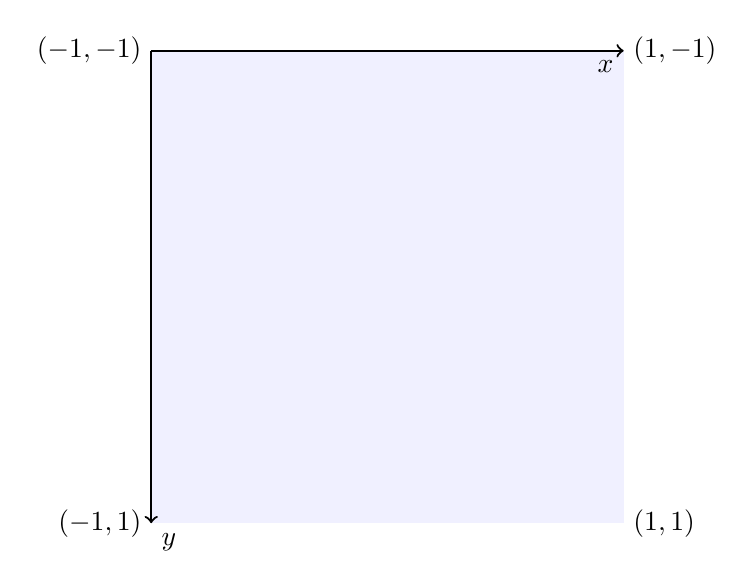
\begin{tikzpicture}[scale=3]
				\coordinate (O) at (0,0,0);
				\coordinate (A) at (2,0,0);
				\coordinate (B) at (0,-2,0);
				\coordinate (C) at (2,-2,0);
				
				
				
				\node at (A) [anchor=west] {$(1,-1)$};
				\node at (B) [anchor=east] {$(-1,1)$};
				\node at (O) [anchor=east] {$(-1,-1)$};
				\node at (C) [anchor=west] {$(1,1)$};
				
				\fill[blue!20,opacity=0.3] (O) -- (A) -- (C) -- (B) -- cycle;
				
				\draw[thick,->] (0,0,0) -- (2,0,0) node[anchor=north east]{$x$};
				\draw[thick,->] (0,0,0) -- (0,-2,0) node[anchor=north west]{$y$};
			\end{tikzpicture}	
		\end{center}
		
		We have omitted the \( z \) axis. It might seem unusual that the \( y \) axis extends from top to bottom. When creating a mathematical model for our engine, we typically use a custom coordinate system and then transform it into this NDC (Normalized Device Coordinates) space. To make this concept clearer, consider the pixel dimensions of your screen. For instance, on a 1920 $\times$ 1080 resolution screen, you can think of the following coordinate system:
		\begin{center}
			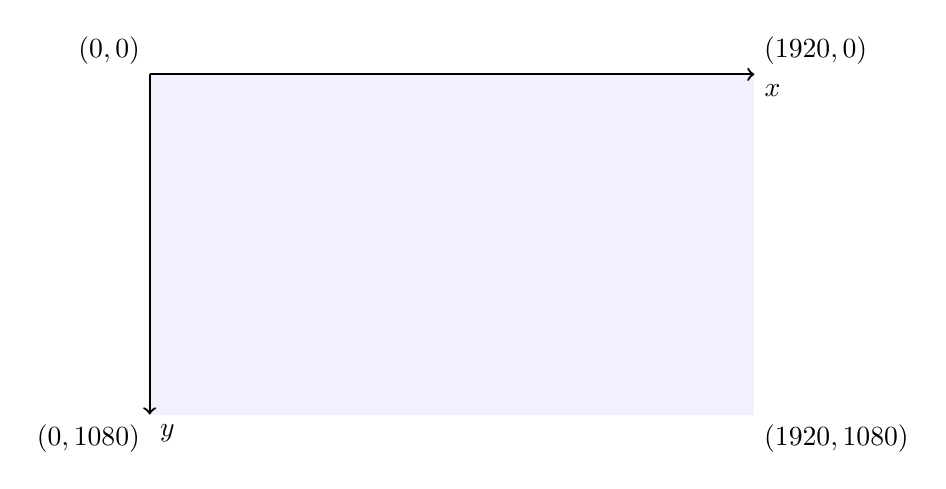
\begin{tikzpicture}[scale=4]
				\coordinate (O) at (0,0,0);
				\coordinate (A) at (1.92,0,0);
				\coordinate (B) at (0,-1.08,0);
				\coordinate (C) at (1.92,-1.08,0);
				
				\node at (A) [anchor=south west] {$(1920,0)$};
				\node at (B) [anchor=north east] {$(0,1080)$};
				\node at (O) [anchor=south east] {$(0,0)$};
				\node at (C) [anchor=north west] {$(1920,1080)$};
				
				\fill[blue!20,opacity=0.3] (O) -- (A) -- (C) -- (B) -- cycle;
				
				\draw[thick,->] (O) -- (B) node[anchor=north west]{$y$};
				\draw[thick,->] (O) -- (A) node[anchor=north west]{$x$};
			\end{tikzpicture}	
		\end{center}
		
		Vulkan will transform the view volume as described above. Each pixel coordinate corresponds to a specific NDC (Normalized Device Coordinates) coordinate. Note that I have intentionally omitted the \( z \) axis here, as understanding the canonical view volume, particularly the \( z \) axis, can be complex. Let's explore this concept further. 
		
		Consider the first vertex, \( p1(0, 0, 0) \). This point is at the center of your screen with a depth value of 0. Next, take the second vertex, \( p2(1, -1, 1) \). This vertex is located at the top-right corner of your screen with a depth value of 1. Lastly, we have \( p3(1, 1, 0.5) \). The triangle formed by these vertices can be visualized as follows:
		
		\begin{center}
			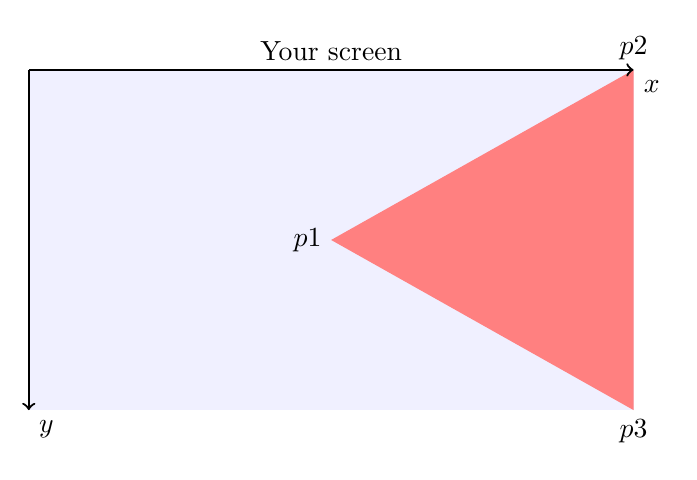
\begin{tikzpicture}[scale=4]
				\coordinate (O) at (0,0,0);
				\coordinate (A) at (1.92,0,0);
				\coordinate (B) at (0,-1.08,0);
				\coordinate (C) at (1.92,-1.08,0);
				
				\coordinate (P1) at (1.92 / 2,-1.08 / 2,0);
				\coordinate (P2) at (1.92,0,0);
				\coordinate (P3) at (1.92,-1.08,0);
				
				\node at (1.92 / 2, 0, 0) [anchor=south] {Your screen};
				
				
				\fill[blue!20,opacity=0.3] (O) -- (A) -- (C) -- (B) -- cycle;
				\fill[red!50,opacity=1] (P1) -- (P2) -- (P3) -- cycle;
				
				\draw[thick,->] (O) -- (B) node[anchor=north west]{$y$};
				\draw[thick,->] (O) -- (A) node[anchor=north west]{$x$};
				
				\node at (P1) [anchor=east] {$p1$};
				\node at (P2) [anchor=south] {$p2$};
				\node at (P3) [anchor=north] {$p3$};
			\end{tikzpicture}
		\end{center}
		
		After the vertex shader outputs these vertices, the \( z \) values will be interpolated at each fragment during the rasterization stage. In the fragment shader, you can even access these interpolated \( z \) values. If a functional depth buffer attachment is set up, Vulkan will use these interpolated values to determine which fragments are visible on top. In this case, the exact \( z \) values of the fragments might not be crucial, but their relative positions to each other are.
		
		\subsection{Local to world}
		Let us start building the model for our object. Note, that this can be done by a lot of different ways. In this case, I am going to use a really simple Cartesian coordinate system where I represent each point of our cube with $p \in \R^3$ point values. \newline
		
		Local coordinate systems:
		\begin{center}
			\tdplotsetmaincoords{60}{30}
			\begin{tikzpicture}[tdplot_main_coords, scale=2]	
				\draw[thick,->] (0,0,0) -- (1.5,0,0) node[anchor=north east]{$x$};
				\draw[thick,->] (0,0,0) -- (0,1.5,0) node[anchor=north west]{$y$};
				\draw[thick,->] (0,0,0) -- (0,0,2.5) node[anchor=south]{$z$};
				
				\coordinate (O) at (0,0,2);
				\coordinate (A) at (1,1,0);
				\coordinate (B) at (-1,1,0);
				\coordinate (C) at (0,-1,0);
				
				\draw (A) -- (B) -- (C) -- cycle;
				\draw (O) -- (B) -- (C) -- cycle;
				\draw (O) -- (A) -- (C) -- cycle;
				\draw (O) -- (B) -- (A) -- cycle;
				
				\fill[blue!20,opacity=0.3] (O) -- (B) -- (C) -- cycle;
				\fill[blue!20,opacity=0.3] (O) -- (A) -- (C) -- cycle;
				\fill[blue!20,opacity=0.3] (O) -- (B) -- (A) -- cycle;
				\fill[blue!20,opacity=0.3] (C) -- (B) -- (A) -- cycle;
				
				\node at (A) [anchor=south west] {$(1,1,0)$};
				\node at (B) [anchor=south east] {$(-1,1,0)$};
				\node at (C) [anchor=south east] {$(0,-1,0)$};
				\node at (O) [anchor=south east] {$(0,0,2)$};
				
				\filldraw[blue!90] (O) circle (1pt);
				\filldraw[blue!90] (A) circle (1pt);
				\filldraw[blue!90] (B) circle (1pt);
				\filldraw[blue!90] (C) circle (1pt);
				
			\end{tikzpicture}
			\tdplotsetmaincoords{60}{30}
			\begin{tikzpicture}[tdplot_main_coords, scale=1.5]	
				\draw[thick,->] (-2,0,0) -- (2,0,0) node[anchor=north east]{$x$};
				\draw[thick,->] (0,-2,0) -- (0,2,0) node[anchor=north west]{$y$};
				\draw[thick,->] (0,0,-2) -- (0,0,2) node[anchor=south]{$z$};
				
				\coordinate (O) at (-1,-1,-1);
				\coordinate (A) at (1,-1,-1);
				\coordinate (B) at (1,1,-1);
				\coordinate (C) at (-1,1,-1);
				\coordinate (D) at (-1,-1,1);
				\coordinate (E) at (1,-1,1);
				\coordinate (F) at (1,1,1);
				\coordinate (G) at (-1,1,1);
				
				% Draw the edges of the cube
				\draw (O) -- (A) -- (B) -- (C) -- cycle; % Bottom face
				\draw (D) -- (E) -- (F) -- (G) -- cycle; % Top face
				\draw (O) -- (D); % Connecting edges
				\draw (A) -- (E);
				\draw (B) -- (F);
				\draw (C) -- (G);
				
				% Optionally, shade the faces
				\fill[blue!20,opacity=0.3] (O) -- (A) -- (E) -- (D) -- cycle;
				\fill[blue!20,opacity=0.3] (A) -- (B) -- (F) -- (E) -- cycle;
				\fill[blue!20,opacity=0.3] (B) -- (C) -- (G) -- (F) -- cycle;
				\fill[blue!20,opacity=0.3] (C) -- (O) -- (D) -- (G) -- cycle;
				\fill[blue!20,opacity=0.3] (D) -- (E) -- (F) -- (G) -- cycle;
				\fill[blue!20,opacity=0.3] (O) -- (A) -- (B) -- (C) -- cycle;
				
				\node at (O) [anchor=north east] {$(-1,-1,-1)$};
				\node at (F) [anchor=south west] {$(1,1,1)$};
				
				\filldraw[blue!90] (O) circle (1pt);
				\filldraw[blue!90] (A) circle (1pt);
				\filldraw[blue!90] (B) circle (1pt);
				\filldraw[blue!90] (C) circle (1pt);
				\filldraw[blue!90] (D) circle (1pt);
				\filldraw[blue!90] (E) circle (1pt);
				\filldraw[blue!90] (F) circle (1pt);
				\filldraw[blue!90] (G) circle (1pt);
				
				\draw[thick] (0,-2,0) -- (0,-1,0);
				\draw[thick] (1,0,0) -- (2,0,0);
			\end{tikzpicture}
		\end{center}
		
		As I mentioned, there might be a lot of different way to model an object. When you start sketching your project, you can think of any model that you find more convenient. However these models all boil down to the same idea of representing object with a finite set of $p \in \R^3$ points, when it comes to placing our object in our world. Here we are, with our set of points:
		\[
		H := \{ p_1, \, p_2, \, p_3, \, p_4, \, p_5, \, p_6 \} \subset \R^3
		\]
		
		We would like to put this cube in our world coordinate system. We use local coordinate systems to determine the shape of our objects  more easily. In these cases our object is usually in the origo. We could have local coordinate systems per object. Now we want to put all of these objects in the world coordinate system that is going to represent our whole space where they live.\newline
		
		We might want to put these in are world.
		\begin{center}
			\tdplotsetmaincoords{60}{30}
			\begin{tikzpicture}[tdplot_main_coords, scale=2]	
				\draw[thick,->] (0,0,0) -- (1.5,0,0) node[anchor=north east]{$x$};
				\draw[thick,->] (0,0,0) -- (0,1.5,0) node[anchor=north west]{$y$};
				\draw[thick,->] (0,0,0) -- (0,0,1.5) node[anchor=south]{$z$};
				
				\coordinate (O) at (1.4651, 0.7248, -0.2000);
				\coordinate (A) at (1.6752, 1.0651, -0.2000);
				\coordinate (B) at (1.3349, 1.2752, -0.2000);
				\coordinate (C) at (1.1248, 0.9349, -0.2000);
				\coordinate (D) at (1.4651, 0.7248, 0.2000);
				\coordinate (E) at (1.6752, 1.0651, 0.2000);
				\coordinate (F) at (1.3349, 1.2752, 0.2000);
				\coordinate (G) at (1.1248, 0.9349, 0.2000);
				
				% Draw the edges of the cube
				\draw (O) -- (A) -- (B) -- (C) -- cycle; % Bottom face
				\draw (D) -- (E) -- (F) -- (G) -- cycle; % Top face
				\draw (O) -- (D); % Connecting edges
				\draw (A) -- (E);
				\draw (B) -- (F);
				\draw (C) -- (G);
				
				\fill[blue!20,opacity=0.3] (O) -- (A) -- (E) -- (D) -- cycle;
				\fill[blue!20,opacity=0.3] (A) -- (B) -- (F) -- (E) -- cycle;
				\fill[blue!20,opacity=0.3] (B) -- (C) -- (G) -- (F) -- cycle;
				\fill[blue!20,opacity=0.3] (C) -- (O) -- (D) -- (G) -- cycle;
				\fill[blue!20,opacity=0.3] (D) -- (E) -- (F) -- (G) -- cycle;
				\fill[blue!20,opacity=0.3] (O) -- (A) -- (B) -- (C) -- cycle;
				
				\coordinate (O) at (1.5, 2.7, 1.1112);
				\coordinate (A) at (2.0556, 3.2556, 0);
				\coordinate (B) at (0.9444, 3.2556, 0);
				\coordinate (C) at (1.5, 2.1444, 0);
				
				
				
				\draw (A) -- (B) -- (C) -- cycle;
				\draw (O) -- (B) -- (C) -- cycle;
				\draw (O) -- (A) -- (C) -- cycle;
				\draw (O) -- (B) -- (A) -- cycle;
				
				\fill[blue!20,opacity=0.3] (O) -- (B) -- (C) -- cycle;
				\fill[blue!20,opacity=0.3] (O) -- (A) -- (C) -- cycle;
				\fill[blue!20,opacity=0.3] (O) -- (B) -- (A) -- cycle;
				\fill[blue!20,opacity=0.3] (C) -- (B) -- (A) -- cycle;
			\end{tikzpicture}
		\end{center}
		
		Let us say we have done that. What about now? Vulkan does not know about 3D vector coordinates. We somehow need to transform the world coordinates to NDC coordinates. It would be convenient to just put our camera somewhere in the world, set its orientation and get the projection of our world somehow. This can actually be straigtforward. Let us start with the camera parameters.
		
		\subsection{Camera}
		
		Here is my camera code that I use:
		\begin{lstlisting}[style=customcpp]
			class Camera
			{
				public:
				Camera(const CameraCreateInfo& createInfo);
				
				glm::mat4 GetViewMatrix()           const;
				glm::mat4 GetProjectionMatrix()     const;
				
				/*
				*  Getters
				*/
				
				private:
				glm::vec3 _position;
				glm::vec3 _worldUp;
				float _fov;
				float _aspect;
				float _yaw;
				float _pitch;
				float _sensitivity;
				float _movementSpeed;
				float _near;
				float _far;
				
				glm::vec3 _front;
				glm::vec3 _right;
				glm::vec3 _up;
				
				void UpdateDirections();
			};
			
		\end{lstlisting}
		
		This is a simple logic for implementing FPS camera movement. Let us go through the variables. I listed the most important pieces of data below:
		
		\begin{itemize}
			\item world position of the camera
			\item up vector of our world
			\item aspect ratio of our frustum
			\item forward facing direction of the camera
			\item up facing direction of the camera
			\item yaw: angle between the forward vector
		\end{itemize}
		
		\begin{center}
			\tdplotsetmaincoords{60}{30}
			\begin{tikzpicture}[tdplot_main_coords, scale=2]	
				\draw[thick,->] (0,0,0) -- (1.5,0,0) node[anchor=north east]{$x$};
				\draw[thick,->] (0,0,0) -- (0,1.5,0) node[anchor=north west]{$y$};
				\draw[thick,->] (0,0,0) -- (0,0,1.5) node[anchor=south]{$z$};
				
				\coordinate (O) at (1.4651, 0.7248, -0.2000);
				\coordinate (A) at (1.6752, 1.0651, -0.2000);
				\coordinate (B) at (1.3349, 1.2752, -0.2000);
				\coordinate (C) at (1.1248, 0.9349, -0.2000);
				\coordinate (D) at (1.4651, 0.7248, 0.2000);
				\coordinate (E) at (1.6752, 1.0651, 0.2000);
				\coordinate (F) at (1.3349, 1.2752, 0.2000);
				\coordinate (G) at (1.1248, 0.9349, 0.2000);
				
				\coordinate (CAM) at (0.5,0.5,2);
				\draw[->] (CAM) -- (1,1,1);
				
				\filldraw[blue!90] (CAM) circle (1pt);
				
				
				% Draw the edges of the cube
				\draw (O) -- (A) -- (B) -- (C) -- cycle; % Bottom face
				\draw (D) -- (E) -- (F) -- (G) -- cycle; % Top face
				\draw (O) -- (D); % Connecting edges
				\draw (A) -- (E);
				\draw (B) -- (F);
				\draw (C) -- (G);
				
				
				\fill[blue!20,opacity=0.3] (O) -- (A) -- (E) -- (D) -- cycle;
				\fill[blue!20,opacity=0.3] (A) -- (B) -- (F) -- (E) -- cycle;
				\fill[blue!20,opacity=0.3] (B) -- (C) -- (G) -- (F) -- cycle;
				\fill[blue!20,opacity=0.3] (C) -- (O) -- (D) -- (G) -- cycle;
				\fill[blue!20,opacity=0.3] (D) -- (E) -- (F) -- (G) -- cycle;
				\fill[blue!20,opacity=0.3] (O) -- (A) -- (B) -- (C) -- cycle;
				
				\coordinate (O) at (1.5, 2.7, 1.1112);
				\coordinate (A) at (2.0556, 3.2556, 0);
				\coordinate (B) at (0.9444, 3.2556, 0);
				\coordinate (C) at (1.5, 2.1444, 0);
				
				
				
				\draw (A) -- (B) -- (C) -- cycle;
				\draw (O) -- (B) -- (C) -- cycle;
				\draw (O) -- (A) -- (C) -- cycle;
				\draw (O) -- (B) -- (A) -- cycle;
				
				\fill[blue!20,opacity=0.3] (O) -- (B) -- (C) -- cycle;
				\fill[blue!20,opacity=0.3] (O) -- (A) -- (C) -- cycle;
				\fill[blue!20,opacity=0.3] (O) -- (B) -- (A) -- cycle;
				\fill[blue!20,opacity=0.3] (C) -- (B) -- (A) -- cycle;
			\end{tikzpicture}
		\end{center}
		
		
		\begin{center}
			\begin{tikzpicture}[scale=2]
				\coordinate (O) at (0,0,0);
				\coordinate (A) at (2,-1,0);
				\coordinate (B) at (2,1,0);
				\draw[thick] (O) -- (A);
				\draw[thick] (O) -- (B);
			\end{tikzpicture}
			
		\end{center}
		
		\begin{center}
			\tdplotsetmaincoords{50}{40}
			\begin{tikzpicture}[tdplot_main_coords, scale=2]
				
				\coordinate (A) at (2,1,1);
				\coordinate (B) at (-2,1,1);
				\coordinate (C) at (2,1,-1);
				\coordinate (D) at (-2,1,-1);			
				\coordinate (O) at (0,-4,0);			
				
				
				\draw (O) -- (A);
				\draw (O) -- (B);
				\draw (O) -- (C);
				\draw (O) -- (D);
				
				\draw (A) -- (B);
				\draw (C) -- (D);
				\draw (A) -- (C);
				\draw (B) -- (D);
				
			\end{tikzpicture}
		\end{center}	
	\end{comment}
	
	
	\section{Convex Mesh Division}
	In this section, I will explain a simple yet effective method to divide any convex polyhedron into arbitrarily small tetrahedrons. This can be useful for creating destructible objects. Let us assume we have a convex polyhedron, where we only know the vertices of each face, and each face can be any polygon.
	
	\subsection{Polyhedron to Tetrahedrons}
	First, we aim to divide our polyhedron into smaller tetrahedrons and subsequently divide those tetrahedrons further. As you might have guessed, a tetrahedron is also a polyhedron. We will use a slightly different approach for dividing tetrahedrons. For simplicity, convert all faces into triangles, which is straightforward:
	
	
	\begin{center}
		\begin{tikzpicture}
			\coordinate (A) at (-5.04,2.68);
			\coordinate (B) at (-5.56,-2.58);
			\coordinate (C) at (2.96,-5.2);
			\coordinate (D) at (4.44,2.12);			
			\coordinate (O) at (-1.22,5.04);
			\draw (A) -- (B) -- (C) -- (D) --(O) -- cycle;
			\draw[dashed] (A) -- (D);
			\draw[dashed] (A) -- (C);
			\node[left] at (A) {$A$};
		\end{tikzpicture}	
	\end{center}
	
	All you need to do is select any vertex $A$ and connect it to every vertex in the polygon except its neighbors.
	
	\begin{lstlisting}[style=customcpp]
		struct Triangle {
			glm::vec3 v1;
			glm::vec3 v2;
			glm::vec3 v3;
		};
		
		std::vector<Triangle> GetTrianglesFromPolygon(const std::vector<glm::vec3>& polygon) {
			std::vector<Triangle> result;
			
			for (int i = 2; i < polygon.size(); ++i) {
				result.push_back(Triangle{polygon[0], polygon[i-1], polygon[i]});
			}
			
			return result;
		}	
	\end{lstlisting}
	
	Now we have any array of triangles that build up our convex polyhedron.
	
	\begin{center}
		\tdplotsetmaincoords{60}{30}
		\begin{tikzpicture}[tdplot_main_coords, scale=2]
			\coordinate (A) at (2,-2,1.2176);
			\coordinate (B) at (-1.78438,-1.21377,1.00766);
			\coordinate (C) at (-3.30891,2.07936,0);
			\coordinate (D) at (0.52544,1.88925,-2);
			\coordinate (E) at (1.51747,-1.44592,-2);
			\coordinate (F) at (-1.72773,-1.47543,-3.02305);
			\coordinate (G) at (1.35119,1.6395,1.69245);
			
			
			
			\draw (A) -- (B) -- (C) -- (G) -- cycle;
			\draw (A) -- (E) -- (F) -- (B) -- (E) -- (G) -- (D) -- (E);
			\draw (A) -- (C);
			\draw[dashed] (D) -- (F) -- (C) -- (D);
			
		\end{tikzpicture}
	\end{center}
	
	The simplest method for dividing a convex polyhedron into smaller tetrahedrons is to find the center of the polyhedron and then connect this center to each of the polyhedron's triangular faces.
	
	\begin{lstlisting}[style=customcpp]
		std::vector<Tetra> GetTetras(const std::vector<Triangle>& triangles) {
			glm::vec3 center{0.0f, 0.0f, 0.0f};
			for (const auto& t : triangles) {
				center += t.v1; center += t.v2; center += t.v3;
			}
			center /= (triangles.size() * 3.0f);
			std::vector<Tetra> tetras;
			for (const auto& t : triangles)
			{
				tetras.push_back({t.v1, t.v2, t.v3, center});
			}
			return tetras;
		}
	\end{lstlisting}
	
	\begin{center}
		\tdplotsetmaincoords{60}{30}
		\begin{tikzpicture}[tdplot_main_coords, scale=2]
			\coordinate (A) at (2,-2,1.2176);
			\coordinate (B) at (-1.78438,-1.21377,1.00766);
			\coordinate (C) at (-3.30891,2.07936,0);
			\coordinate (D) at (0.52544,1.88925,-2);
			\coordinate (E) at (1.51747,-1.44592,-2);
			\coordinate (F) at (-1.72773,-1.47543,-3.02305);
			\coordinate (G) at (1.35119,1.6395,1.69245);
			\coordinate (M) at (-0.204,-0.075,-0.444);
			
			
			\draw (A) -- (B) -- (C) -- (G) -- cycle;
			\draw (A) -- (E) -- (F) -- (B) -- (E) -- (G) -- (D) -- (E);
			\draw (A) -- (C);
			\draw[dashed] (D) -- (F) -- (C) -- (D);
			
			\draw[dotted] (A) -- (M);
			\draw[dotted] (B) -- (M);
			\draw[dotted] (C) -- (M);
			\draw[dotted] (D) -- (M);
			\draw[dotted] (E) -- (M);
			\draw[dotted] (F) -- (M);
			\draw[dotted] (G) -- (M);
			
		\end{tikzpicture}
	\end{center}
	
	
	\subsection{Tetrahedrons to tetrahedrons}
	We have successfully divided our mesh into tetrahedrons. While further subdivision might be desirable, this method may not be the most effective for dividing the tetrahedrons themselves. Let's explore why this particular tetrahedron could be an example of our polyhedron:
	
	\begin{center}
		\tdplotsetmaincoords{60}{10}
		\begin{tikzpicture}[tdplot_main_coords, scale=1.5]
			\coordinate (A) at (-1.48478,-2.47241,0);
			\coordinate (B) at (-2,3,-0.1549);
			\coordinate (C) at (2.6, 0, 0);
			\coordinate (D) at (0, 0, 3);
			
			
			\draw (A) -- (B) -- (D) -- (A) -- (C) -- (D);
			\draw[dashed] (B) -- (C);
			
			
			\node[below] at (A) {$A$};
			\node[left] at (B) {$B$};
			\node[right] at (C) {$C$};
			\node[above] at (D) {$D$};
			
			
		\end{tikzpicture}
	\end{center}
	
	As illustrated, continuing this pattern would result in all the sub-tetrahedrons having identical faces. This would produce very thin tetrahedrons with wide faces, which might not be ideal for our purposes. Therefore, let’s explore a different algorithm. Our overall goal is to calculate the midpoints of all the edges in each tetrahedron and use these midpoints to generate smaller tetrahedrons.
	
	\begin{center}
		\tdplotsetmaincoords{60}{10}
		\begin{tikzpicture}[tdplot_main_coords, scale=1.5]
			\coordinate (A) at (-1.48478,-2.47241,0);
			\coordinate (B) at (-2,3,-0.1549);
			\coordinate (C) at (2.6, 0, 0);
			\coordinate (D) at (0, 0, 3);
			
			\coordinate (AB) at (-1.74239,0.263795,-0.07745);
			\coordinate (AC) at (0.55761,-1.236205,0);
			\coordinate (AD) at (-0.74239,-1.236205,1.5);
			\coordinate (BC) at (0.3,1.5,-0.07745);
			\coordinate (BD) at (-1,1.5,1.42255);
			\coordinate (CD) at (1.3,0,1.5);
			
			\draw (A) -- (B) -- (D) -- (A) -- (C) -- (D);
			\draw[dashed] (B) -- (C);
			
			
			\node[below] at (A) {$A$};
			\node[left] at (B) {$B$};
			\node[right] at (C) {$C$};
			\node[above] at (D) {$D$};
			
			\draw[dotted] (AC) -- (AB) -- (AD) -- cycle;
			\draw[dotted] (BD) -- (CD) -- (AD) -- cycle;
			\draw[dotted] (AC) -- (BC) -- (CD) -- cycle;
			\draw[dotted] (AB) -- (BC) -- (BD) -- cycle;
			\draw[dotted] (BC) -- (AD);
		\end{tikzpicture}
	\end{center}
	
	The illustration may be tricky, but there are actually eight smaller tetrahedrons within the larger one. Identifying the vertices is straightforward:
	
	\begin{center}
		\tdplotsetmaincoords{60}{10}
		\begin{tikzpicture}[tdplot_main_coords, scale=1.5]
			\coordinate (A) at (-1.48478,-2.47241,0);
			\coordinate (AB) at (-1.74239,0.263795,-0.07745);
			\coordinate (AC) at (0.55761,-1.236205,0);
			\coordinate (AD) at (-0.74239,-1.236205,1.5);
			
			\node[below] at (A) {$A$};
			\node[left] at (AB) {$AB$};
			\node[right] at (AC) {$AC$};
			\node[above] at (AD) {$AD$};
			
			\draw[dashed] (AB) -- (AC);
			\draw (AB) -- (A) -- (AC) -- (AD) -- (AB);
			\draw (AD) -- (A);
		\end{tikzpicture}
		\tdplotsetmaincoords{60}{10}
		\begin{tikzpicture}[tdplot_main_coords, scale=1.5]
			\coordinate (B) at (-2,3,-0.1549);
			
			\coordinate (AB) at (-1.74239,0.263795,-0.07745);
			\coordinate (BC) at (0.3,1.5,-0.07745);
			\coordinate (BD) at (-1,1.5,1.42255);
			
			\node[left] at (B) {$B$};
			\node[left] at (AB) {$AB$};
			\node[right] at (BC) {$BC$};
			\node[above] at (BD) {$BD$};
			
			
			\draw[dashed] (B) -- (BC);
			\draw (BC) -- (BD) -- (B) -- (AB);
			\draw (BD) -- (AB) -- (BC);
		\end{tikzpicture}
		
		\tdplotsetmaincoords{60}{10}
		\begin{tikzpicture}[tdplot_main_coords, scale=1.5]
			\coordinate (C) at (2.6, 0, 0);
			
			\coordinate (AC) at (0.55761,-1.236205,0);
			\coordinate (BC) at (0.3,1.5,-0.07745);
			\coordinate (CD) at (1.3,0,1.5);
			
			\node[right] at (C) {$C$};
			\node[left] at (AC) {$AC$};
			\node[left] at (BC) {$BC$};
			\node[above] at (CD) {$CD$};
			
			
			\draw[dashed] (BC) -- (C);
			\draw (BC) -- (AC) -- (C) -- (CD) -- (BC);
			\draw (AC) -- (CD);
		\end{tikzpicture}
		\tdplotsetmaincoords{60}{10}
		\begin{tikzpicture}[tdplot_main_coords, scale=1.5]
			\coordinate (D) at (0, 0, 3);
			
			\coordinate (AD) at (-0.74239,-1.236205,1.5);
			\coordinate (BD) at (-1,1.5,1.42255);
			\coordinate (CD) at (1.3,0,1.5);
			
			\node[above] at (D) {$D$};
			\node[left] at (BD) {$BD$};
			\node[right] at (CD) {$CD$};
			\node[left] at (AD) {$AD$};
			
			\draw[dashed] (BD) -- (CD);
			\draw (BD) -- (D) -- (CD) -- (AD) -- (BD);
			\draw (AD) -- (D);
		\end{tikzpicture}
	\end{center}
	
	Within the tetrahedron, there is a hexahedron comprised of four tetrahedrons.
	
	\begin{center}
		\tdplotsetmaincoords{70}{-5}
		\begin{tikzpicture}[tdplot_main_coords, scale=1.5]
			\coordinate (AB) at (-1.74239,0.263795,-0.07745);
			\coordinate (AC) at (0.55761,-1.236205,0);
			\coordinate (AD) at (-0.74239,-1.236205,1.5);
			\coordinate (BC) at (0.3,1.5,-0.07745);
			\coordinate (BD) at (-1,1.5,1.42255);
			\coordinate (CD) at (1.3,0,1.5);
			
			\node[left] at (AB) {$AB$};
			\node[below] at (AC) {$AC$};
			\node[left] at (AD) {$AD$};
			\node[right] at (BC) {$BC$};
			\node[above] at (BD) {$BD$};
			\node[right] at (CD) {$CD$};
			
			
			\draw (AB) -- (BD) -- (AD) -- (AB);
			\draw (AD) -- (AC) -- (CD) -- (AD);
			\draw (AB) -- (AC);
			\draw (BD) -- (CD);
			
			\draw[dashed] (AB) -- (BC);
			\draw[dashed] (AC) -- (BC);
			\draw[dashed] (AD) -- (BC);
			\draw[dashed] (BD) -- (BC);
			\draw[dashed] (CD) -- (BC);
		\end{tikzpicture}
	\end{center}
	
	The algorithm is quite straightforward. You start with six vertices and need to select two that do not share a common vertex. Following this labeling approach, if you examine the labels of the chosen midpoints, they will encompass all the vertices. In this case, the appropriate pairs of vertices might be:
	\[
	AD - BC, \, AB - CD, \, BD - AC
	\]
	All four tetrahedrons will contain these two vertices. Next, we need to determine the order in which to assemble the remaining four vertices. For instance, if we choose \(AD\) and \(BC\) as the two vertices, the tetrahedrons should be assembled as follows:
	
	\begin{enumerate}
		\item $AD, \, BC, \, \cdot, \, \cdot$
		\item $AD, \, BC, \, \cdot, \, \cdot$
		\item $AD, \, BC, \, \cdot, \, \cdot$
		\item $AD, \, BC, \, \cdot, \, \cdot$
	\end{enumerate}
	
	where the $\cdot$ symbols represent the remaining vertices. The algorithm is also quite simple: you need to choose two vertices that share exactly one vertex.
	
	
	\begin{enumerate}
		\item $AD, \, BC, \, B\mathbf{D}, \, C\mathbf{D}$
		\item $AD, \, BC, \, \mathbf{B}D, \, A\mathbf{B}$
		\item $AD, \, BC, \, \mathbf{A}B, \, \mathbf{A}C$
		\item $AD, \, BC, \, A\mathbf{C}, \, \mathbf{C}D$
	\end{enumerate}
	
	\begin{center}
		\tdplotsetmaincoords{70}{-5}
		\begin{tikzpicture}[tdplot_main_coords, scale=1.5]
			\coordinate (AD) at (-0.74239,-1.236205,1.5);
			\coordinate (BC) at (0.3,1.5,-0.07745);
			\coordinate (AB) at (-1.74239,0.263795,-0.07745);
			\coordinate (BD) at (-1,1.5,1.42255);
			
			\node[left] at (AD) {$AD$};
			\node[right] at (BC) {$BC$};
			\node[below] at (AB) {$AB$};
			\node[above] at (BD) {$BD$};
			
			\draw (AD) -- (AB) -- (BD) -- cycle;
			\draw (BD) -- (BC) -- (AB);
			\draw (AD) -- (BC);
		\end{tikzpicture}
		\tdplotsetmaincoords{70}{-5}
		\begin{tikzpicture}[tdplot_main_coords, scale=1.5]
			\coordinate (AD) at (-0.74239,-1.236205,1.5);
			\coordinate (BC) at (0.3,1.5,-0.07745);
			
			\coordinate (BD) at (-1,1.5,1.42255);
			\coordinate (CD) at (1.3,0,1.5);
			
			\node[left] at (AD) {$AD$};
			\node[below] at (BC) {$BC$};
			\node[left] at (BD) {$BD$};
			\node[right] at (CD) {$CD$};
			
			\draw (BD) -- (CD) -- (AD) -- cycle;
			\draw (AD) -- (BC) -- (CD);
			\draw[dashed] (BD) -- (BC);
		\end{tikzpicture}
		
		\tdplotsetmaincoords{70}{-5}
		\begin{tikzpicture}[tdplot_main_coords, scale=1.5]
			\coordinate (AD) at (-0.74239,-1.236205,1.5);
			\coordinate (BC) at (0.3,1.5,-0.07745);
			\coordinate (AB) at (-1.74239,0.263795,-0.07745);
			\coordinate (AC) at (0.55761,-1.236205,0);
			
			
			\node[above] at (AD) {$AD$};
			\node[above right] at (BC) {$BC$};
			\node[left] at (AB) {$AB$};
			\node[below right] at (AC) {$AC$};
			
			\draw (AB) -- (AD) -- (AC) -- cycle;
			\draw (AD) -- (BC) -- (AC);
			\draw[dashed] (AB) -- (BC);
		\end{tikzpicture}
		\tdplotsetmaincoords{70}{-5}
		\begin{tikzpicture}[tdplot_main_coords, scale=1.5]
			\coordinate (AD) at (-0.74239,-1.236205,1.5);
			\coordinate (BC) at (0.3,1.5,-0.07745);
			\coordinate (AC) at (0.55761,-1.236205,0);
			\coordinate (CD) at (1.3,0,1.5);
			
			\node[left] at (AD) {$AD$};
			\node[right] at (BC) {$BC$};
			\node[below] at (AC) {$AC$};
			\node[right] at (CD) {$CD$};
			
			\draw (AD) -- (CD) -- (AC) -- cycle;
			\draw[dashed] (AD) -- (BC) -- (CD);
			\draw[dashed] (BC) -- (AC);
			
			
		\end{tikzpicture}
	\end{center}
	
	The good news is that the midpoints calculated initially do not need to be exact; they can be any points along the edges. This flexibility can lead to a noisy division.
	
	\subsection{Triangle vertex ordering}
	In computer graphics, the ordering of triangle vertices is really important. When you look at your mesh at any position in the world, the triangles you are currently looking at have to be ordered either clockwise or counter clokwise. In this subsection I provide as simple algorithm to order the triangles in your mesh. Let us have a list of triangles that built up our mesh. Using the glm library here is a code:
	
	\begin{lstlisting}[style=customcpp]
bool IsClockwise(const Triangle& triangle, const glm::vec3& polyCenter)
{
	glm::vec3 triangleCenter = (triangle.v1 + triangle.v2 + triangle.v3) / 3.0f;
	glm::vec3 outVector = triangleCenter - polyCenter;
	
	glm::vec3 v1 = outVector.v2 - outVector.v1;
	glm::vec3 v2 = triangle.v3 - triangle.v1;
	glm::vec3 normal = glm::cross(v1, v2);
	
	return glm::dot(normal, outVector) > 0;
}
	\end{lstlisting}
	Now let us dvelve into this code with illustrations. Let we have a convex polyhedron. We can easily calculate it's centerpoint by adding up all the vertices and then dividing with the size. For simplicity I have chosen a tetrahedron:
	
	\begin{center}
		\tdplotsetmaincoords{60}{0}
		\begin{tikzpicture}[tdplot_main_coords, scale=1.5]
			\coordinate (A) at (-1.48478,-2.47241,0);
			\coordinate (B) at (-2,3,-0.1549);
			\coordinate (C) at (2.6, 0, 0);
			\coordinate (D) at (0, 0, 3);
			
			\coordinate (M) at (-0.221195,0.1318975,0.711275);
			\coordinate (CENTER) at (0.37173,-0.82414,1);
			\coordinate (NORMAL) at (0.472,-0.780,0.410);
			
			\draw (A) -- (B) -- (D) -- (A) -- (C) -- (D);
			\draw[dashed] (B) -- (C);
			
			\filldraw [black] (M) circle (2pt);
			
			
			\draw[->, thick] (M) -- (CENTER);
			\draw[->, thick] (M) -+ (CENTER) --+(NORMAL);
			
			\node[below] at (A) {$A$};
			\node[left] at (B) {$B$};
			\node[right] at (C) {$C$};
			\node[above] at (D) {$D$};
			
			
		\end{tikzpicture}
	\end{center}
	
	
	
\end{document}